\begin{frame}\frametitle{How did we do it?}
  \setbeamercovered{invisible}
  \begin{columns}
    \begin{column}{0.4\linewidth}
      \begin{block}{Tasks:}
        \begin{itemize}
          \item Implement $K_{ij}$, $G_{ij}$
          \item Convenience functions
          \item 2d integration
          \item 2d interpolation
          \item Maris-Tandy
          \item Quark $M,\, A$
        \end{itemize}
      \end{block}
    \end{column}
    \pause
    \begin{column}{0.2\linewidth}
      \centering
      $\rightarrow$
    \end{column}
    \begin{column}{0.4\linewidth}
      \begin{block}{New tasks:}
        \begin{itemize}
          \item Iteration
          \item Calculate $K'_{ij}$
          \item File output
          \item Optimize
        \end{itemize}
      \end{block}
    \end{column}
  \end{columns}
  \pause
  \begin{tikzpicture}[remember picture,overlay]
    \node[anchor=south west,inner sep=0pt,text width=10cm] at ($(current page.south west)+(5.2cm,5.99cm)$) {
      \fontsize{12}{14}\selectfont\textcolor{black}{Around two days...}
    };
  \end{tikzpicture}
  \pause
  \begin{tikzpicture}[remember picture,overlay]
    \node[anchor=south west,inner sep=0pt] at ($(current page.south west)+(8.2cm,6.1cm)$) {
      
\includegraphics[width=0.18\linewidth]{Important.jpeg}
    };
  \end{tikzpicture}
  \begin{tikzpicture}[remember picture,overlay]
    \node[anchor=south west,inner sep=0pt,text width=10cm] at ($(current page.south west)+(7.2cm,1.0cm)$) {
      \fontsize{30}{35}\selectfont\textcolor{red}{\textbf{Bugs.}}
    };
  \end{tikzpicture}
\end{frame}

\begin{frame}\frametitle{Bugs}
  \setbeamercovered{invisible}
  {\Large Collective Bughunt:}


  {\small
    \begin{tikzpicture}[remember picture,overlay]
      \node[anchor=south west,inner sep=0pt] at ($(current page.south west)+(7.2cm,5.5cm)$) {
        
\includegraphics[width=0.3\linewidth]{frog.png}
      };
    \end{tikzpicture}

    \pause
    \vspace{3mm}
    Divisions by zero

    \pause
    \vspace{3mm}
    We found bugs in Normalization $\rightarrow$ factor $2(2\pi)^4 \approx 10^3$

    \pause
    \vspace{3mm}
    Forgot Jacobi determinant

    \pause
    \vspace{3mm}
    Mismatched some indices
  }
\end{frame}

\begin{frame}\frametitle{Stupid numerics}
  \setbeamercovered{invisible}
  \begin{columns}
    \centering
    \begin{column}{0.4\linewidth}
      \begin{block}{}
        \vspace{-0.cm}
        But still no convergence, everything goes to $\infty$...
      \end{block}
    \end{column}
    \pause
    \begin{column}{0.2\linewidth}
      \centering
      {\tiny
        Some parameter testing...\\
      }
      $\rightarrow$
    \end{column}
    \pause
    \begin{column}{0.4\linewidth}
      \begin{block}{Numerics issue}
        \vspace{-0.cm}
          Oversampled UV tail
      \end{block}
    \end{column}
  \end{columns}
  \pause
  \vspace{1cm}
  \centering
  $\Rightarrow$ Logarithmic grid for $k^2$
\end{frame}

\begin{frame}\frametitle{Program overview}
  \tiny
      \begin{figure}
        \begin{forest}
          for tree={
            align=center,
            font=\sffamily,
            edge+={thin, -{[]}},
            l sep'+=10pt,
            fork sep'=10pt,
          },
          forked edges,
          if level=0{
            inner xsep=0pt,
            tikz={\draw [thin] (.children first) -- (.children last);}
          }{},
          [Quark\_Photon\_Vertex
            [Simulation.cpp
              [iteration.hh
                [
                [quark\_dse.hh]
                [Kernels\_G.hh]
                [Kernels\_K.hh]
                [maris\_tandy.hh]
                ]
                [
                [
                [quark\_model\_functions.hh]
                [basistransform.hh]
                [momentumtransform.hh]
                ]
                ]
              ]
              [parameters.hh]
              [types.hh]
              [fileIO.hh]
            ]
          ]
        \end{forest}
      \end{figure}
      \begin{figure}
        \begin{forest}
          for tree={
            align=center,
            font=\sffamily,
            edge+={thin, -{[]}},
            l sep'+=10pt,
            fork sep'=10pt,
          },
          forked edges,
          if level=0{
            inner xsep=0pt,
            tikz={\draw [thin] (.children first) -- (.children last);}
          }{},
          [core
            [PolynomialBase.hh
              [LegendrePolynomials.hh]
            ]
            [LinearInterpolate.hh]
            [QuadratureIntegral.hh]
            [Utils.hh]
          ]
        \end{forest}
      \end{figure}
\end{frame}

\begin{frame}\frametitle{Program flow}
  \begin{block}{Workflow for fixed $Q$}
    \begin{figure}
      \small
      \tikzstyle{startstop} = [rectangle, rounded corners, minimum width=2cm, minimum height=0.7cm,text centered, draw=black, fill=red!30]
      \tikzstyle{process} = [rectangle, minimum width=2cm, minimum height=0.7cm, text centered, draw=black, fill=orange!30]
      \tikzstyle{decision} = [rectangle, minimum width=2cm, minimum height=0.7cm, text centered, draw=black, fill=green!30]
      \tikzstyle{arrow} = [thick,->,>=stealth]
      \tikzstyle{arrow} = [->,>=stealth]
      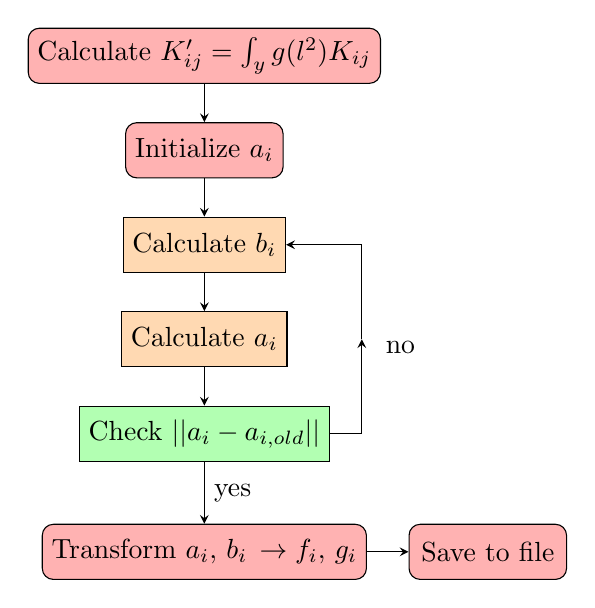
\begin{tikzpicture}[node distance=2cm]
        \node (start) [startstop] {Calculate $K'_{ij} = \int_y g(l^2) K_{ij}$};
        \node (start2) [startstop, below of=start, yshift=0.8cm] {Initialize $a_i$};
        \draw [arrow] (start) -- (start2);
        \node (pro1) [process, below of=start2, yshift=0.8cm] {Calculate $b_i$};
        \draw [arrow] (start2) -- (pro1);
        \node (pro2) [process, below of=pro1, yshift=0.8cm] {Calculate $a_i$}; \coordinate[right of=pro2] (empty);
        \draw [arrow] (pro1) -- (pro2);
        \node (pro3) [decision, below of=pro2, yshift=0.8cm] {Check $||a_i - a_{i,\text{old}}||$};
        \draw [arrow] (pro2) -- (pro3);
        \draw [arrow] (pro3) -| node[anchor=east,yshift=1.1cm,xshift=0.8cm] {no} (empty);
        \draw [arrow] (empty) |- (pro1);
        \node (transform) [startstop, below of=pro3, yshift=0.5cm] {Transform $a_i,\,b_i\,\rightarrow f_i,\,g_i$};
        \draw [arrow] (pro3) -- node[anchor=west] {yes} (transform);
        \node (save) [startstop, right of=transform, xshift=1.6cm] {Save to file};
        \draw [arrow] (transform) -- (save);
      \end{tikzpicture}
    \end{figure}
  \end{block}
\end{frame}

\endinput